\documentclass[crop,tikz]{standalone}
\usepackage{tikz,pgfplots}
\usetikzlibrary{calc,shapes}

% @author Thomas Prest
% @author Pierre-Alain Fouque
% @author Jeffrey Hoffstein
% @author Paul Kirchner
% @author Vadim Lyubashevsky
% @author Thomas Pornin
% @author Thomas Ricosset
% @author Gregor Seiler
% @author William Whyte
% @author Zhenfei Zhang
% @copyright The authors


\definecolor{coral}{RGB}{255,87,40}
\definecolor{cblue}{RGB}{31, 117, 254}
\definecolor{mantis}{RGB}{116, 195, 101}
\definecolor{shamrock}{RGB}{0, 158, 96}
\definecolor{emerald}{RGB}{80, 200, 120}
\definecolor{france}{RGB}{49, 140, 231}
\definecolor{gold}{RGB}{249,196,95}
\definecolor{klein}{RGB}{0,46,167}
\definecolor{ultramarine}{RGB}{63,0,255}
\definecolor{navy}{RGB}{0,0,128}
\definecolor{midnight}{RGB}{25,25,112}
\definecolor{burgundy}{RGB}{144, 0, 32}

%%%%%%%%%%%%%%%%%%%%%%%%%%%%%%%%%%%%%%%%%%%%%%%%%%%%%%%%%%%%
\colorlet{one}{gold}
\colorlet{two}{black!60!cblue}
% \colorlet{two}{midnight}
\colorlet{three}{gold!20}
\colorlet{four}{black!20!cblue!20}
\colorlet{five}{shamrock}


\colorlet{color_cite}{burgundy}
\colorlet{color_url}{navy}
\colorlet{color_link}{navy}


\tikzstyle{point}=[circle,scale=0.3,fill=black]
\tikzstyle{cpoint}=[circle,scale=0.3,fill=red,draw=black]


 %%%%%%%%%%
 %FFO
 %%%%%%%%%%
\newcommand{\largeur}{150mm}
\newcommand{\hauteur}{8mm}
\tikzstyle{case}=[rectangle, thin, minimum width=\largeur, minimum height=\hauteur, draw = black, fill=white, inner sep = 0cm, anchor=south west]
\newcommand{\da}[2]{ \draw[->] (C#1.south) -> (C#2.north); }

\begin{document}

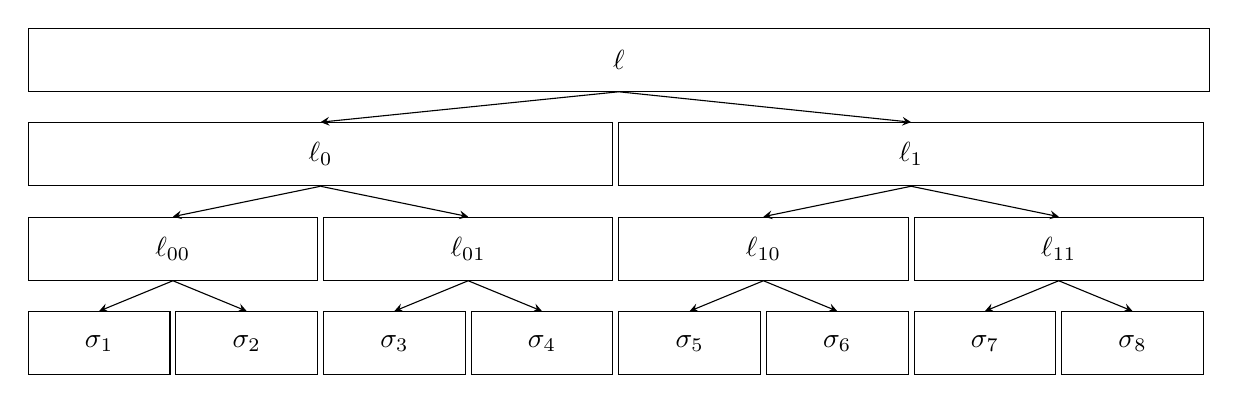
\begin{tikzpicture}[>=stealth]

 \node[case,minimum width=\largeur] (C) at (0,0) {$\ell$};

 \foreach \i in {0,1}%
 {%
     \node[case,minimum width=0.495*\largeur] (C\i) at (0.5*\i*\largeur,-1.5*\hauteur) {$\ell_\i$};%
     \da{}{\i};
     \foreach \k in {0,1}{
         \node[case,minimum width=0.245*\largeur] (C\i\k) at (0.25*\k*\largeur+0.5*\i*\largeur,-3*\hauteur) {$\ell_{\i\k}$};
         \da{\i}{\i\k};
          \foreach \l in {0,1}{
             \node[case,minimum width=0.12*\largeur] (C\i\k\l) at (0.25*\k*\largeur+0.5*\i*\largeur+0.125*\l*\largeur,-4.5*\hauteur) {$\sigma_{\i\k\l}$};
             \da{\i\k}{\i\k\l};
         }
     }
 }

 \foreach \l in {1,...,8}{
 \node[case,minimum width=0.12*\largeur] at (0.125*\l*\largeur-0.125*\largeur,-4.5*\hauteur) {$\sigma_\l$};
 }


\end{tikzpicture}

\end{document}

